%==========================================================
%
% Formalizing Theorems with PVS
%
% Summer UnB
%
% Jan 17 - 21, 2022
%
%==========================================================
%==========================================================
\documentclass[10pt]{beamer}
\usepackage[utf8]{inputenc}
%\usepackage[brazil]{babel}
\usepackage{multicol}
\usepackage{amssymb}
\usepackage{amsmath}
\usepackage{graphicx}
\usepackage{xcolor}
\usepackage{mathtools}
\usepackage{mathrsfs}
\usepackage{fancyvrb}
\usepackage[all,2cell]{xy}
\usepackage{proof}  
\usepackage{mathpartir}
\usepackage{tikz}
\usetikzlibrary{arrows,snakes,backgrounds}
\usepackage{pdfsync}
\synctex=1

%==========================================================
%==========================================================
\usecolortheme[cmyk={0.8,0.3,0,0.6}]{structure}
    \usetheme[secheader]{Boadilla}         
    \setbeamertemplate{footline}
        {
      \leavevmode%
      \hbox{%
\begin{beamercolorbox}[wd=.333333\paperwidth,ht=2.25ex,dp=1ex,center]{author in head/foot}%
        \usebeamerfont{author in head/foot}\insertshortauthor~~%(\insertshortinstitute)
      \end{beamercolorbox}%
\begin{beamercolorbox}[wd=.333333\paperwidth,ht=2.25ex,dp=1ex,center]{title in head/foot}%
        \usebeamerfont{title in head/foot}\insertshorttitle
      \end{beamercolorbox}%
\begin{beamercolorbox}[wd=.333333\paperwidth,ht=2.25ex,dp=1ex,right]{date in head/foot}%
        \usebeamerfont{date in head/foot}\insertshortdate{}\hspace*{2em}
      \end{beamercolorbox}}%
      \vskip0pt%
    }
\usefonttheme[onlymath]{serif}
\setbeamertemplate{theorems}[numbered]    
%==========================================================
%==========================================================
%==========================================================
\newtheorem{teorema}{Teorema}[section]
\newtheorem{corolario}[teorema]{Corol\'{a}rio}
\newtheorem{lema}[teorema]{Lema}
\newtheorem{proposicao}[teorema]{Proposi\c{c}\~{a}o}
\newcommand{\demonstracao}{\noindent {\color{red}{Demonstra\c{c}\~{a}o:}} }
\newtheorem{definicao}[teorema]{Defini\c{c}\~{a}o}
%==========================================================
\newtheorem{exemplo}{Exemplo}[section]
\newtheorem{exemplos}[exemplo]{Exemplos}
\newtheorem{nota}{Nota}[section]
\newtheorem{observacao}[nota]{Observa\c{c}\~{a}o}
\newtheorem{notacao}[nota]{Nota\c{c}\~{a}o}
%==========================================================
%==========================================================
%==========================================================
\newcommand{\bck}[0]{$\backslash$}
\newcommand{\ttblue}[1]{{\color{blue!80!black}\tt#1}}
\newcommand{\ttbe}[1]{{\color{blue!80!black}\tt\emph{#1}}}
\definecolor{aquamarine}{rgb}{0.5, 1.0, 0.83}
\definecolor{darkorange}{rgb}{1.0, 0.55, 0.0}
\newcommand{\op}[1]{_{\scriptscriptstyle{#1}}}
\newcommand{\ttdo}[1]{{\color{darkorange}\tt#1}}
\newcommand{\ttaq}[1]{{\color{aquamarine}\tt#1}}
\newcommand{\boxdarkgray}[1]{\fbox{\color{darkgray}{#1}}}
\linespread{1.3}
%==========================================================
% new commands ISR2018
%==========================================================
\newcommand{\deriv}{\bigtriangledown}
\newcommand{\cut}{\mm{(Cut)}}
\newcommand{\toesm}{\mm{(\to_e)}}
\newcommand{\toism}[1]{\mm{(\to_i){#1}}}
\newcommand{\toe}{\mm{(\to_e)}}
\newcommand{\toisa}{\mm{(\to_i)}}
\newcommand{\toi}[1]{\mm{(\to_i)\;{#1}}}
\newcommand{\landi}{\mm{(\land_i)}}
\newcommand{\lande}{\mm{(\land_e)}}
\newcommand{\landef}{\mm{(\land_{e_1})}}
\newcommand{\landes}{\mm{(\land_{e_2})}}
\newcommand{\lorif}{\mm{(\lor_{i_1})}}
\newcommand{\loris}{\mm{(\lor_{i_2})}}
\newcommand{\lori}{\mm{(\lor_i)}}
\newcommand{\lore}[2]{\mm{(\lor_e)\;{#1},{#2}}}
\newcommand{\loresa}{\mm{(\lor_e)}}
\newcommand{\loresm}[2]{\mm{(\lor_e)\;{#1},{#2}}}
\newcommand{\nege}{\mm{(\neg_e)}}
\newcommand{\negi}[1]{\mm{(\neg_i)\;{#1}}}
\newcommand{\negisa}{\mm{(\neg_i)}}
\newcommand{\nne}{\mm{(\neg\neg_e)}}
\newcommand{\nni}{\mm{(\neg\neg_i)}}
\newcommand{\nnesm}{\mm{(\neg\neg_e)}}
\newcommand{\nnism}{\mm{(\neg\neg_i)}}
\newcommand{\lem}{\rm{LEM}}
\newcommand{\pair}[2]{\mm{\langle #1, #2 \rangle}}
\newcommand{\pbc}[1]{\mm{({\rm PBC})\;{#1}}}
\newcommand{\pbcsm}[1]{(\rm{PBC}),#1}
\newcommand{\pbcsa}{(\rm{PBC})}
\newcommand{\lemcp}{(\rm{LEM})}
\newcommand{\mt}{\rm{MT}}
\newcommand{\bote}{\mm{(\bot_e)}}
\newcommand{\botesm}{\mm{(\bot_e)}}
\newcommand{\nat}{\mm{\mathbb{N}}}
\newcommand{\add}{\mm{\tt +}}
\newcommand{\lb}{\mm{\lambda}}
\newcommand{\alle}{\mm{(\forall_e)}}
\newcommand{\alli}{\mm{(\forall_i)}}
\newcommand{\exie}[1]{\mm{(\exists_e)\;{#1}}}
\newcommand{\exii}{\mm{(\exists_i)}}
\newcommand{\true}{\mm{ T}}
\newcommand{\false}{\mm{ F}}
\newcommand{\m}{{\tt m}}
\newcommand{\z}{{\tt z}}
\newcommand{\pseq}{\mbox{{\tt |---}\;}} 

\newcommand{\var}{{\sc (Var)}}
\newcommand{\app}{{\sc (App)}}
\newcommand{\absA}{{\sc (Abs)}}
\newcommand{\imp}{\to}
\newcommand{\axiom}{{\sc (axiom)}} 
\newcommand{\axiomvar}{{\sc (axiom\ var)}} 
\newcommand{\axiomtop}{{\sc (axiom\ $\top$)}} 
\newcommand{\axiombot}{{\sc (axiom\ $\bot$)}} 
\newcommand{\negation}{{\sc (negation)}} 
\newcommand{\conjunction}{{\sc (conjunction)}} 
\newcommand{\disjunction}{{\sc (disjunction)}} 
\newcommand{\implication}{{\sc (implication)}} 
\newcommand{\prop}{\rm{Prop}}
\newcommand{\tvarset}{\mathbb{V}}
\newcommand{\funset}{\mathbb{F}}
\newcommand{\predset}{\mathbb{P}}
\newcommand{\dom}{\mm{\tt D}}
\newcommand{\fv}[1]{{\tt fv}(#1)}
\newcommand{\bv}[1]{{\tt bv}(#1)}
\newcommand{\set}[1]{ \{ #1 \}}
\renewcommand{\min}[1]{ {min \{ #1 \}}}
\newcommand{\vars}[1]{\mm{{\tt var}(#1)}}
\newcommand{\subs}[2]{ \{ #1/#2 \}}
\newcommand{\fosubs}[2]{ [#1/#2]}




% Begin Commands Talk Verao 2007
\newcommand{\myboxvariable}[3]{\vspace{-3mm}$$\vbox{\hrule\hbox{\vrule\hskip#1\vbox{\vskip#1{}\hsize=#2\hsize\noindent#3\vskip#1}\hskip#1\vrule}\hrule}\vspace{-3.7mm}$$}
\newcommand\mdc{\mbox{\it gcd}}
\newcommand\LDB{\Lambda_{dB}}
\newcommand{\fd}{\to}
\newcommand{\abst}[3]{\lambda {#1}{:}{#2}.{#3}}
\newcommand\FV{{\mathcal FV}}
\newcommand\sub[3]{{#1}\{{#2}/{#3}\}}
\newcommand{\SEL}[1]{(\lambda #1)}
\newcommand{\SEA}[2]{(#1\;#2)}
\newcommand{\SEDB}[1]{{\tt \underline{#1}}}
\newcommand{\SEVr}[1]{#1}
\newcommand{\SESb}[2]{#1[#2]}
\newcommand{\SES}[3]{(#2\sigma^{#1}#3)}
\newcommand{\SEP}[3]{\varphi^{#1}_{#2}(#3)}
\newcommand{\SEDummy}{\diammond}
\newcommand{\SESp}[4]{[\![#1,#2,#3,#4]\!]}
\newcommand{\SEId}{id}
\newcommand{\SEUp}{\uparrow}
\newcommand{\SEPt}[2]{(#1\cdot #2)}
\newcommand{\SECp}[2]{(#1\circ#2)}
\newcommand{\SECon}[2]{#1::#2}
\newcommand{\SECk}[4]{\{\!\{#1,#2,#3,#4\}\!\}}
\newcommand{\SENil}{nil}
\newcommand{\SEPaar}[2]{(#1,#2)}
\newcommand{\SEAr}[1]{@#1}
\newcommand{\SELG}[4]{\langle\!\langle#1,#2,#3,#4\rangle\!
angle}


\newcommand{\rTo}{\longrightarrow}

\newcommand{\abs}[2]{\lambda_{#1}.{#2}}
\newcommand{\absG}[2]{\mbox{\color{\FigGcol}$\lambda_{#1}.{#2}$}}
\newcommand{\absR}[2]{\mbox{\color{\FigRcol}$\lambda_{#1}.{#2}$}}
\newcommand{\absB}[2]{\mbox{\color{\FigBcol}$\lambda_{#1}.{#2}$}}
\newcommand{\tyabs}[2]{\lambda_{#1}.{#2}}
\newcommand{\absb}[1]{\lambda.{#1}}
\newcommand{\absbG}[1]{\mbox{\color{\FigGcol}$\lambda.{#1}$}}
\newcommand{\absbR}[1]{\mbox{\color{\FigRcol}$\lambda.{#1}$}}
\newcommand{\absbB}[1]{\mbox{\color{\FigBcol}$\lambda.{#1}$}}
\newcommand{\absdb}[1]{\lambda {#1}}
\newcommand{\apl}[2]{({#1}\;\;{#2})}
\newcommand{\myigls}{=_{\lambda s_e}^?}
\newcommand{\igls}{=_{\lambda\sigma}^?}
\newcommand{\tvar}{{\it {\cal T}var}}
\newcommand\Sub[2]{{#1}[{#2}]}
\newcommand\Id{id}
\newcommand\Comp[2]{{#1} \circ {#2}}
\newcommand\Sh{\uparrow}
\newcommand{\substit}{{\it Subst}}
\newcommand{\vvar}{{\it var}}
\newcommand{\fvar}{{\it {\cal F}var}}
\newcommand{\beigls}{=_{\beta\eta}^?}
\newcommand \si {\,\sigma^i}
\newcommand \fik {\varphi^i_k}
\newcommand{\AND}{\ {\wedge}\ }
\newcommand{\OR}{\ {\vee}\ }
\newcommand{\IMPLIES}{\ {\Rightarrow}\ }
\newcommand{\NOT}{\neg}

%==========================================================

\title
[Mechanizing Mathematics]
{\vspace{-5mm}
%\includegraphics[scale=.35]{Marca_UFG.png}
\\%[8mm]
%{\scriptsize\bf  Universidad Nacional de Colombia - Sede Manizales}\\
{\bf\Large Mechanizing Mathematics}\\
{\large The Prototype Verification System vs Sequent Calculus}  \vspace{-.1cm}}


\author[M. Ayala-Rinc\'on (UnB) \& T. A. de Lima (UFG)]
{Universidad Nacional de Colombia - Sede Manizales \\
Facultad de Ciencias Exactas y Naturales\\[6mm]
\textbf{Thaynara Arielly de Lima
  (IME)}   
\includegraphics[scale=.18]{../1_Intr_Math_Deduction/ufg.png}\\
\textbf{Mauricio Ayala-Rinc\'on (CIC-MAT)} 
\includegraphics[scale=.03]{../1_Intr_Math_Deduction/unb.jpg}
\vspace{-.8cm}}

\date[Universidad Nacional de Colombia - Sede Manizales]{{\scriptsize\it Funded by the Brazilian agencies CNPq, grants Universal 409003/21-2; \\ FAPDF, grant DE 00193-00001175/2021-11 and \\ FAPEG, grant 202310267000223.}
\\ May 29 - June 02 ,
  2023}  



\pgfdeclareimage[height=2.0cm]{deBruijn}{../1_Intr_Math_Deduction/figs/deBruijn}
\pgfdeclareimage[height=2.0cm]{Landau}{../1_Intr_Math_Deduction/figs/EdmundLandau}
\pgfdeclareimage[height=3.5cm]{35Years}{../1_Intr_Math_Deduction/figs/35YearsAutomath}
\pgfdeclareimage[height=1cm]{35YearsA}{../1_Intr_Math_Deduction/figs/35YearsAutomath}
\pgfdeclareimage[height=3.5cm]{SelectedAutomath}{../1_Intr_Math_Deduction/figs/SelectedAutomath}
\pgfdeclareimage[height=2cm]{CurryHoward}{../1_Intr_Math_Deduction/figs/CurryHoward}
\pgfdeclareimage[height=1cm]{AutomathHeader}{../1_Intr_Math_Deduction/figs/AutomathHeader}
\pgfdeclareimage[height=2.5cm]{KnuthSelectedPapersonAlgorithms}{../1_Intr_Math_Deduction/figs/KnuthSelectedPapersonAlgorithms}
\pgfdeclareimage[height=2.5cm]{KnuthdeBruijn}{../1_Intr_Math_Deduction/figs/KnuthdeBruijn}
\pgfdeclareimage[height=2.0cm]{VladimirVoevodsky}{../1_Intr_Math_Deduction/figs/VladimirVoevodsky} 
\pgfdeclareimage[height=0.8cm]{FieldMedal}{../1_Intr_Math_Deduction/figs/FieldMedal} 
\pgfdeclareimage[height=2.5cm]{GrundlageAnalysiscapa}{../1_Intr_Math_Deduction/figs/GrundlageAnalysiscapa}
\pgfdeclareimage[height=3.5cm]{HottBook}{../1_Intr_Math_Deduction/figs/HottBook} 
\pgfdeclareimage[height=3.5cm]{ITPcapa}{../1_Intr_Math_Deduction/figs/ITPcapa} 
\pgfdeclareimage[height=3.5cm]{MSCScapa}{../1_Intr_Math_Deduction/figs/MSCScapa} 
\pgfdeclareimage[height=3.5cm]{TCScapa}{../1_Intr_Math_Deduction/figs/TCScapa} 
\pgfdeclareimage[height=3.5cm]{JARcapa}{../1_Intr_Math_Deduction/figs/JARcapa} 
\pgfdeclareimage[height=3.5cm]{LJIGPLcapa}{../1_Intr_Math_Deduction/figs/LJIGPLcapa} 
\pgfdeclareimage[height=3.5cm]{SCPcapa}{../1_Intr_Math_Deduction/figs/SCPcapa}
\pgfdeclareimage[height=3.5cm]{SciComProgCover}{../1_Intr_Math_Deduction/figs/SciComProgCover}
\pgfdeclareimage[height=3.5cm]{WoLLICcapa}{../1_Intr_Math_Deduction/figs/WoLLICcapa} 
\pgfdeclareimage[height=3.5cm]{ENTCScapa}{../1_Intr_Math_Deduction/figs/ENTCScapa} 
\pgfdeclareimage[height=3.5cm]{LOPSTRcapa}{../1_Intr_Math_Deduction/figs/LOPSTRcapa} 
\pgfdeclareimage[height=3.5cm]{LMCScapa}{../1_Intr_Math_Deduction/figs/LMCScapa}
\pgfdeclareimage[height=3.1cm]{LogforCScapa}{../1_Intr_Math_Deduction/figs/LogforCScapa}
\pgfdeclareimage[height=3.1cm]{Logiccapa}{../1_Intr_Math_Deduction/figs/Logiccapa} 
\pgfdeclareimage[height=3.1cm]{ProofTheorycapa}{../1_Intr_Math_Deduction/figs/ProofTheorycapa} 
\pgfdeclareimage[height=3.1cm]{TypeTheorycapa}{../1_Intr_Math_Deduction/figs/TypeTheorycapa} 
\pgfdeclareimage[height=3.1cm]{Rewritingcapa}{../1_Intr_Math_Deduction/figs/Rewritingcapa} 

\pgfdeclareimage[height=0.5cm]{LIPIcscapita}{../1_Intr_Math_Deduction/figs/LIPIcsCapa}
\pgfdeclareimage[height=0.5cm]{ITPcapita}{../1_Intr_Math_Deduction/figs/ITPcapa}
\pgfdeclareimage[height=0.5cm]{SciComProgCapita}{../1_Intr_Math_Deduction/figs/SciComProgCover}
\pgfdeclareimage[height=0.5cm]{MSCScapita}{../1_Intr_Math_Deduction/figs/MSCScapa} 
\pgfdeclareimage[height=0.5cm]{TCScapita}{../1_Intr_Math_Deduction/figs/TCScapa} 
\pgfdeclareimage[height=0.5cm]{JARcapita}{../1_Intr_Math_Deduction/figs/JARcapa} 
\pgfdeclareimage[height=0.5cm]{LJIGPLcapita}{../1_Intr_Math_Deduction/figs/LJIGPLcapa} 
\pgfdeclareimage[height=0.5cm]{SCPcapita}{../1_Intr_Math_Deduction/figs/SCPcapa} 
\pgfdeclareimage[height=0.5cm]{WoLLICcapita}{../1_Intr_Math_Deduction/figs/WoLLICcapa} 
\pgfdeclareimage[height=0.5cm]{ENTCScapita}{../1_Intr_Math_Deduction/figs/ENTCScapa} 
\pgfdeclareimage[height=0.5cm]{LOPSTRcapita}{../1_Intr_Math_Deduction/figs/LOPSTRcapa} 
\pgfdeclareimage[height=0.5cm]{LMCScapita}{../1_Intr_Math_Deduction/figs/LMCScapa} 

%==========================================================
%==========================================================
\begin{document}
%==========================================================
%==========================================================
\begin{frame}
\maketitle
\end{frame}
%==========================================================
%==========================================================
\begin{frame}
\frametitle{Talk's Plan}
%----------------------------------------
\begin{columns}
\begin{column}{10cm}
%----------------------------------------
\tableofcontents
%----------------------------------------
\end{column}
\end{columns}
%----------------------------------------
\end{frame}






\section{The Prototype Verification System (PVS)}

\begin{frame}
\frametitle{ The Prototype Verification System (PVS)}
%----------------------------------------
\begin{columns}
\begin{column}{10cm}
%----------------------------------------

%\begin{block}{}
{\color{red} PVS} is a verification system, developed by the SRI International Computer Science Laboratory, which consists of

\begin{enumerate}

\item a \emph{\color{red} specification language}:


\begin{itemize}

\item based on \emph{higher-order logic};

\item a type system based on Church's simple theory of types
augmented with \emph{subtypes} and \emph{dependent types}.
\end{itemize}

\item an \emph{\color{red} interactive theorem prover}:

\begin{itemize}

\item based on {\bf sequent calculus}; that is, goals in PVS are
sequents of the form \boldmath{$\Gamma \vdash \Delta$}, where $\Gamma$ and
$\Delta$ are finite sequences of formulae, with the usual Gentzen
semantics.
\end{itemize}
\end{enumerate} 
%\end{block}

%----------------------------------------
\end{column}
\end{columns}
%----------------------------------------
\end{frame}
%==========================================================
%==========================================================
\begin{frame}
\frametitle{The Prototype Verification System (PVS) | Libraries }
%----------------------------------------
\begin{columns}
\begin{column}{11cm}
%----------------------------------------
\begin{itemize}
\item {\color{red}The {\tt prelude} library} 
\begin{itemize}
\item It is a collection of basic \emph{theories} containing specifications about:
\begin{itemize}
\item functions;
\item sets;
\item predicates;
\item logic; among others.
\end{itemize}
\item The theories in the prelude library are visible in all PVS contexts;
\item It provides the infrastructure for the PVS typechecker and prover, as well as much of the basic mathematics needed to support specification and verification of systems.
\end{itemize} 
\end{itemize}

%----------------------------------------
\end{column}
\end{columns}
%----------------------------------------
\end{frame}
%==========================================================
%==========================================================
\begin{frame}
\frametitle{The Prototype Verification System (PVS) | Libraries }
%----------------------------------------
\begin{columns}
\begin{column}{11cm}
%----------------------------------------
\begin{itemize}
\item {\color{red}NASA LaRC PVS library ({\tt nasalib})} 
\begin{itemize}
\item It includes the \emph{theories}
\begin{itemize}
\item {\color{blue}structures}, analysis, algebra, graphs, {\color{blue}digraphs}, 
\item real arithmetic, floating point arithmetic, {\color{blue}groups}, interval arithmetic,
\item linear algebra, measure integration, metric spaces, 
\item orders, probability, series, sets, topology, 
\item {\color{blue}term rewriting systems}, {\color{blue}unification}, etc. etc.
\end{itemize}
\item The {\tt nasalib} is maintaned by the NASA LaRC formal methods group;
\item The {\tt nasalib} is result of research developed by the
  NASA LaRC formal methods group and the cientific comunity in
  general.
\end{itemize}
\end{itemize}

%----------------------------------------
\end{column}
\end{columns}
%----------------------------------------
\end{frame}
%==========================================================
%==========================================================
\begin{frame}
\frametitle{Sequent Calculus in PVS}
%----------------------------------------
A sequent of the form {\color{red} $\Gamma\vdash\Delta$} (or {\color{red}$A_1,A_2,...,A_n\vdash
B_1,B_2,...,B_m$}, since $\Gamma$ and $\Delta$ are finite sequences
of formulae) is:
\vspace{.2cm}

{\small
 \begin{minipage}{.53\textwidth}
        \begin{itemize}
\item interpreted as: \\{\footnotesize{\color{red}$A_1\AND A_2\AND ...\AND A_n\vdash
    B_1\OR B_2\OR ...\OR B_m$}}, that is, from the conjunction of the
  antecedent formulae one obtains the disjunction of the succedent
  formulae. 
\end{itemize}
\end{minipage}%
}
\hfill\vline\hfill
{\small
 \begin{minipage}{.43\textwidth}
        \begin{itemize}
\item represented in PVS as: 
	{\color{blue}\begin{center}
			\begin{tabular}{c}
				\small{\tt{[-1] $A_1$}} \\ \small{\tt{$\vdots$}} \\ \small{\tt{[-n] $A_n$}} \\ \small{\tt{|----------}}
				\\ \small{\tt{[1] $B_1$}} \\ \small{\tt{$\vdots$}} \\ \small{\tt{[m] $B_m$}}
			\end{tabular} 
		\end{center}}
\end{itemize}
\end{minipage}%
}

%----------------------------------------
\end{frame}
%==========================================================
%==========================================================
\begin{frame}
\frametitle{Sequent Calculus in PVS}
%----------------------------------------

 \begin{minipage}{.49\textwidth}

        \begin{itemize}

\item Inference rules
		\begin{itemize} {\footnotesize
			\item Premises and conclusions are simultaneously constructed:\vspace{1mm}
			   \[\dfrac{\Gamma\vdash\Delta}{\Gamma'\vdash\Delta'}\]
                        \item A PVS proof command corresponds to the application of an inference rule.
		 In general: 
			
			\mbox{}\hspace{3cm}$\infer[ \textbf{(Rule Name)}]{\Gamma_1\vdash\Delta_1...\Gamma_n\vdash\Delta_n}{\Gamma\vdash\Delta}$
}	
		\end{itemize}
		\item Goal: $\vdash \Delta$.
\end{itemize}
\end{minipage}%
\hfill\vline\hfill
{\small
 \begin{minipage}{.5\textwidth}
        \begin{itemize}
\item {\small Proof tree: each node is labelled by a sequent}
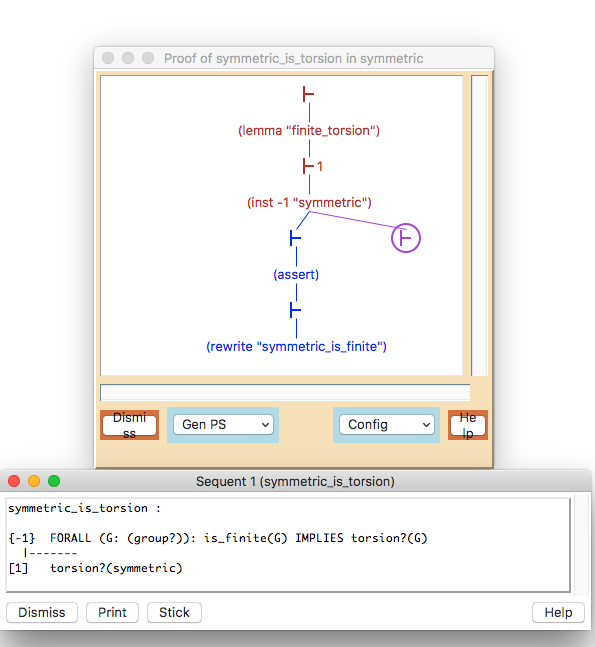
\includegraphics[scale=.27]{tree_example.png}
\end{itemize}
\end{minipage}%
}

%----------------------------------------
\end{frame}
%==========================================================
%==========================================================
\begin{frame}
\frametitle{Some inference rules in PVS}
%----------------------------------------

 	\begin{itemize}
		\item \underline{{\color{blue}Structural}}:
{\scriptsize
\begin{table}
\vspace{-7mm}
\[\begin{array}{|c@{\hspace{1cm}}c|}
\hline
\mbox{\footnotesize Deduction rule} & \mbox{\footnotesize PVS command} \\
\hline
&\\
\infer[(LC\mbox{\it ontraction})]{\varphi,\Gamma\Rightarrow\Delta}{\varphi,\varphi,\Gamma\Rightarrow\Delta} & 
\infer[(copy)]{\varphi,\varphi,\Gamma\vdash\Delta}{\varphi,\Gamma\vdash\Delta}\\[3mm]
\hline
\end{array}\]
\end{table}
}

{\footnotesize
\[\begin{array}{l}
     \hspace{10mm}\vdots\\
     \,[-i]\; A \wedge \neg B \\
     \hspace{10mm}\vdots\\
     {\small{\tt{|------}}} \\
     \hspace{10mm} \vdots\\
     \,[j]\;  \neg C\rightarrow D \\
     \hspace{10mm} \vdots\\
   \end{array}         
   \hspace{1mm}
   \begin{array}{c}{\color{red}{\tt (copy -i)}} \hspace{6mm}\rightsquigarrow\end{array}
   \hspace{10mm}
   \begin{array}{l}
     \,{\color{blue}[-1]\; A \wedge \neg B} \\
     \hspace{10mm}\vdots\\
     \,{\color{blue}[-(i+1)]\; A \wedge \neg B} \\
     \hspace{10mm}\vdots\\
    {\small{\tt{|------}}} \\
     \hspace{10mm} \vdots\\
     \,[j]\;  \neg C\rightarrow D \\
     \hspace{10mm} \vdots\\
   \end{array}  \]
}

\end{itemize}

%----------------------------------------
\end{frame}

%==========================================================
%==========================================================
\begin{frame}
\frametitle{Some inference rules in PVS}
	\begin{itemize}
		\item \underline{{\color{blue}Structural}}:
{\scriptsize
\begin{table}
\vspace{-7mm}
\[\begin{array}{|c@{\hspace{1cm}}c|}
\hline
\mbox{\footnotesize Deduction rule} & \mbox{\footnotesize PVS command} \\
\hline
&\\
\infer[(LW\mbox{\it eakening})]{\varphi,\Gamma\Rightarrow\Delta}{\Gamma\Rightarrow\Delta} & 
\infer[(hide)]{\Gamma\vdash\Delta}{\varphi,\Gamma\vdash\Delta} \\[3mm]
\hline
\end{array}\]
\end{table}
}

{\footnotesize
\[\begin{array}{l}
    \,[-1]\; A \wedge \neg B \\
    \hspace{10mm}\vdots\\
    \,{\color{blue}[-(i+1)]\; A \wedge \neg B} \\
    \hspace{10mm}\vdots\\
     {\small{\tt{|------}}}\\
    \hspace{10mm} \vdots\\
    \,[j]\;  \neg C\rightarrow D \\
    \hspace{10mm} \vdots\\
  \end{array}      
  \hspace{1mm}
  \begin{array}{c}{\color{red}{\tt (hide -(i+1))}}\hspace{6mm}\rightsquigarrow\end{array}
  \hspace{10mm}
  \begin{array}{l}
    \,[-1]\; A \wedge \neg B \\
    \hspace{10mm}\vdots\\
     {\small{\tt{|------}}} \\
    \hspace{10mm} \vdots\\
    \,[j]\;  \neg C\rightarrow D \\
    \hspace{10mm} \vdots\\
  \end{array}         
  \]
}

\end{itemize}
\end{frame}
%==========================================================
%==========================================================

\begin{frame}
	\frametitle{Some inference rules in PVS}
\begin{itemize}
\item \underline{{\color{blue}Propositional}}:

\begin{minipage}{.48\textwidth}
{\small
\[\begin{array}{l}
     {\small{\tt{|------}}} \\[1mm]
     \,[1]\;  A \wedge B \rightarrow (C \vee D \rightarrow C \vee  (A
    \wedge C)) \\[1mm]
    \hspace{20mm}\downarrow {\color{red}{\tt (flatten)}}\\[2mm]
   %\end{array}         
   %\hspace{2mm}
   %\begin{array}{l}{\tt (flatten)}\end{array}
   %\hspace{2mm}
   %\begin{array}{l}
     \,[-1]\; A  \\[1mm]
     \,[-2]\; B \\[1mm]
     \,[-3]\; C \vee D \\[1mm]
     {\small{\tt{|------}}} \\[1mm]
     \,[1]\; C \\[1mm]
     \,[2]\; A \wedge C 
   \end{array}      
   \] 
}
\end{minipage}
%\hfill\vfill\hfill
\begin{minipage}{.4\textwidth}
{\scriptsize
\begin{table}
\vspace{-7mm}
\[\begin{array}{|c@{\hspace{.3cm}}c|}
\hline
\mbox{\footnotesize Deduction rule} & \mbox{\footnotesize PVS command} \\
& {\color{red}(flatten)} \\
\hline
&\\
\infer[(R_\rightarrow)]{\Gamma\Rightarrow\Delta,\varphi\rightarrow\psi}{\varphi,\Gamma\Rightarrow\Delta,
  \psi} &
\infer[]{\varphi,\Gamma\vdash\Delta, \psi}{\Gamma\vdash\Delta,\varphi\rightarrow\psi}\\[5mm]
\infer[(L_\wedge)]{\varphi_1\wedge\varphi_2,\Gamma\Rightarrow\Delta}{\varphi_{1},\varphi_{2},\Gamma\Rightarrow\Delta} & 
\infer[]{\varphi_{i\in\{1,2\}},\Gamma\vdash\Delta}{\varphi_1\wedge\varphi_2,\Gamma\vdash\Delta} \\[5mm]
\infer[(R_\vee)]{\Gamma\Rightarrow\Delta,\varphi_1\vee\varphi_2}{\Gamma\Rightarrow\Delta,
  \varphi_{i\in\{1,2\}} }&
\infer[]{\Gamma\vdash\Delta, \varphi_{1}, \varphi_{2}}{\Gamma\vdash\Delta,\varphi_1\vee\varphi_2}\\[3mm]
\hline
\end{array}\]
\end{table}
}
\end{minipage}
\end{itemize}
\end{frame}
%==========================================================
%==========================================================

\begin{frame}
	\frametitle{Some inference rules in PVS}
\begin{itemize}
\item \underline{{\color{blue}Propositional}}:
{\scriptsize
\begin{table}
\vspace{-5mm}
\[\begin{array}{|c@{\hspace{1cm}}c|}
\hline
\mbox{\footnotesize Deduction rule} & \mbox{\footnotesize PVS command} \\
\hline
&\\
\infer[(L_\rightarrow)]{\varphi\rightarrow\psi,\Gamma\Rightarrow\Delta}{\Gamma\Rightarrow\Delta,\varphi\;\;\psi,\Gamma\Rightarrow\Delta} & 
\infer[(split)]{\Gamma\vdash\Delta,\varphi\;\;\psi,\Gamma\vdash\Delta}{\varphi\rightarrow\psi,\Gamma\vdash\Delta} \\[3mm]
\hline
\end{array}\]
\end{table}
}

\[\begin{array}{clc}
   & \,[-\!1]\; (A\rightarrow B)\rightarrow A&\\[1mm]
    &{\small{\tt{|------}}} \hspace{5mm}{\color{red}{\tt (split -\!1) }}& \\[1mm]
   & \,[1]\;  A & \\
  \swarrow& & \searrow \\[3mm]
\begin{array}{l}
 \,[-1]\; A  \\[1mm]
    {\small{\tt{|------}}} \\[1mm]
    \,[1]\; A 
\end{array} & & 
\begin{array}{l}
{\small{\tt{|------}}} \\[1mm]
    \,[1]\; A \rightarrow B \\[1mm]
    \,[2]\; A 
\end{array} 
   \end{array}         
  %\hspace{1mm}
  %\begin{array}{c}{\color{red}{\tt (split -\!1) }}\end{array}
  % \hspace{3mm}
  % \begin{array}{l}
  %   \,[-1]\; A  \\[1mm]
  %   {\small{\tt{|------}}} \\[1mm]
  %   \,[1]\; A \\[8mm]
  %   {\small{\tt{|------}}} \\[1mm]
  %   \,[1]\; A \rightarrow B \\[1mm]
  %   \,[2]\; A 
  %\end{array}      
  \]

\end{itemize}
\end{frame}

%==========================================================
%==========================================================

\begin{frame}
	\frametitle{Some inference rules in PVS}
\begin{itemize}
\item \underline{{\color{blue}Propositional}}:
{\small
\[\hspace{-1.2cm}\begin{array}{l}
     {\small{\tt{|------}}} \hspace{ 4mm}{\color{red}{\tt (case \;``m \geq n") }}\\[1mm]
    \,[1]\; \gcd(m,n) = \gcd(n,m)
  \end{array}         
  \hspace{.2cm}
  \begin{array}{c} \rightsquigarrow\end{array} 
\hspace{.2cm}
  \begin{array}{l}
    \,{\color{blue}[-\!1]\;  m \geq n} \\[1mm]
     {\small{\tt{|------}}} \\[1mm]
    \,[1]\; \gcd(m,n) = \gcd(n,m)\\[10mm]
     {\small{\tt{|------}}} \\[1mm]
    \,{\color{blue}[1]\;  m \geq n} \\[1mm]
    \,[2]\; \gcd(m,n) = \gcd(n,m)
  \end{array}      
  \]
}
\end{itemize}
\end{frame}

%==========================================================
%==========================================================

\frame{
	\frametitle{Some inference rules in PVS}
\begin{itemize}
\item \underline{{\color{blue}Propositional}} - semantics of PVS instructions:


  \[\displaystyle\infer[{\color{red}{\tt (split)}}]{\Gamma\pseq \Delta,  \mbox{\bf if $a$ then $b$ else $c$ endif} } 
    { \infer[{\color{red}{\tt (flatten)}}]{\Gamma\pseq \Delta,  a \rightarrow b}{a,
        \Gamma\pseq\Delta,   b}  & & &  \infer[{\color{red}{\tt (flatten)}}]{\Gamma\pseq\Delta,  \neg a \rightarrow c}{\Gamma\pseq\Delta,  a, c}
    }\]


\[\infer[{\color{red}{\tt (split)}}]{ \mbox{\bf if $a$ then $b$ else $c$ endif}, \Gamma \pseq\Delta   }
    { \infer[{\color{red}{\tt (flatten)}}]{ a \wedge b, \Gamma\pseq\Delta
      }{a,b,\Gamma \pseq\Delta }  & & &  \infer[{\color{red}{\tt (flatten)}}]{\neg
        a \wedge c, \Gamma\pseq\Delta  }{c,\Gamma\pseq\Delta,  a}
    } \]


\end{itemize}

}
%==========================================================
%==========================================================
\begin{frame}
	\frametitle{Some inference rules in PVS}

	\begin{itemize}
		\item \underline{{\color{blue}Propositional}} {\color{red}(propax)}:
\vspace{3mm}
		\begin{center}
		\boxdarkgray{$\infer[\textbf{(Ax)}]{\mbox{}}{\Gamma,A\pseq A,\Delta}$}\hspace{10mm}
			\boxdarkgray{$\infer[\textbf{(FALSE} \pseq \textbf{)}]{\mbox{}}{\Gamma,FALSE\vdash\Delta}$}
		
			\vspace{10mm}
			
			\boxdarkgray{$\infer[\textbf{(} \vdash \textbf{TRUE)}]{\mbox{}}{\Gamma\pseq TRUE,\Delta}$}
		\end{center}	
	\end{itemize}
\end{frame}

%==========================================================
%==========================================================

%==========================================================
%==========================================================
\begin{frame}
\frametitle{Some inference rules in PVS}
%----------------------------------------

 	\begin{itemize}
		\item \underline{{\color{blue}Predicate}}:
{\scriptsize
\begin{table}
\vspace{-7mm}
\[\begin{array}{|c@{\hspace{1cm}}c|}
\hline
\mbox{\footnotesize Deduction rule} & \mbox{\footnotesize PVS command} \\
\hline
&\\
\infer[(L_\exists),\;\;\;y\not\in \fv{\Gamma,\Delta}]{\exists_x\varphi,\Gamma\Rightarrow\Delta}{\varphi[x/y],\Gamma\Rightarrow\Delta} & 
\infer[(skolem),\;\;\;y\not\in \fv{\Gamma,\Delta}]{\varphi[x/y],\Gamma\vdash\Delta}{\exists_x\varphi,\Gamma\vdash\Delta} \\[3mm]
\infer[(L_\forall)]{\forall_x \varphi, \Gamma\Rightarrow\Delta}{\varphi[x/t],\Gamma\Rightarrow\Delta} & 
\infer[(inst)]{\varphi[x/t],\Gamma\vdash\Delta}{\forall_x \varphi, \Gamma\vdash\Delta}\\[3mm]
\hline
\end{array}\]
\end{table}
}
{\small	
\[\begin{array}{l}
    \,[-\!1]\; \forall_{x:T} : P(x)  \\[1mm]
    \,{\color{blue}[-\!2]\;    \exists_{x:T} : \neg P(x)} \\[1mm]
    \pseq 
  \end{array}         
  %\hspace{.5cm}
  \begin{array}{c}{\color{red}{\tt (skolem -\! 2 \,``z")} } \hspace{.5cm} \rightsquigarrow \end{array} \hspace{1cm}
  \begin{array}{l}
    \,[-\!1]\; \forall_{x:T} : P(x)  \\[1mm]
    \pseq \\[1mm]
    \,{\color{blue}[1]\; P(z)} \\
  \end{array}         
  \]
\hrulefill
\[ \begin{array}{l}
    \,{\color{blue}[-\!1]\; \forall_{x:T} : P(x) } \\[1mm]
    \pseq \\[1mm]
    \,[1]\; P(z) 
  \end{array}         
  \begin{array}{c}{\color{red}{\tt (inst -\! 1\, ``z") }} \hspace{.5cm} \rightsquigarrow\end{array} \hspace{1cm}
\left(\begin{array}{c}
    \,{\color{blue}[-\!1]\;  P(z) } \\[1mm]
    \pseq \\[1mm]
    \,[1]\; P(z) \end{array} \right)
 \begin{array}{l} {\tt Q.E.D.}
  \end{array}      
  \]
}


\end{itemize}

%----------------------------------------
\end{frame}

%==========================================================
%==========================================================



%==========================================================
%==========================================================

\subsection{Gentzen Deductive Rules vs PVS Proof Commands}
\frame{
\frametitle{Summary - Gentzen Deductive Rules  vs  Proof Commads}
\vspace{-7mm}
{\footnotesize
\begin{table}
\caption{\textsc{Structural Left Rules vs Proof Commands}}
\vspace{-7mm}
\[\begin{array}{|c@{\hspace{1cm}}c|}
\hline
& \\
\mbox{\footnotesize Structural left rules} & \mbox{\footnotesize PVS commands} \\[2mm]
\hline
& \\[2mm]
\infer[(LW\mbox{\it eakening})]{\varphi,\Gamma\Rightarrow\Delta}{\Gamma\Rightarrow\Delta} & 
\infer[(hide)]{\Gamma\vdash\Delta}{\varphi,\Gamma\vdash\Delta} \\[5mm]
\infer[(LC\mbox{\it ontraction})]{\varphi,\Gamma\Rightarrow\Delta}{\varphi,\varphi,\Gamma\Rightarrow\Delta} & 
\infer[(copy)]{\varphi,\varphi,\Gamma\vdash\Delta}{\varphi,\Gamma\vdash\Delta}\\[5mm]
\hline


\hline
\end{array}\]
\end{table}
}

}

%==========================================================
%==========================================================
\frame{
\frametitle{Summary - Gentzen Deductive Rules  vs  Proof Commads}
\vspace{-7mm}
{\footnotesize
\begin{table}
\caption{\textsc{Structural Right Rules vs Proof Commands}}
\vspace{-7mm}
\[\begin{array}{|c@{\hspace{1cm}}c|}
\hline
& \\
\mbox{\footnotesize Structural right rules} & \mbox{\footnotesize PVS commands} \\[2mm]
\hline
& \\[2mm]
\infer[(RW\mbox{\it eakening})]{\Gamma\Rightarrow\Delta,\varphi}{\Gamma\Rightarrow\Delta}
& 
\infer[(hide)]{\Gamma\vdash\Delta}{\Gamma\vdash\Delta,\varphi}\\[5mm]
\infer[(RC\mbox{\it ontraction})]{\Gamma\Rightarrow\Delta,\varphi}{\Gamma\Rightarrow\Delta,\varphi,\varphi}&
\infer[(copy)]{\Gamma\vdash\Delta,\varphi,\varphi}{\Gamma\vdash\Delta,\varphi}\\[5mm]
\hline


\hline
\end{array}\]
\end{table}
}

}




\frame{
\frametitle{Summary -  Gentzen Deductive Rules  vs  Proof Commads}
\vspace{-4mm}
{\tiny
\begin{table}
\caption{\textsc{Logical Left Rules vs Proof Commands}}
\vspace{-7mm}
\[\begin{array}{|c@{\hspace{1cm}}c|}
\hline
& \\
\mbox{\footnotesize Left rules} & \mbox{\footnotesize PVS commands} \\[2mm]
\hline
& \\[2mm]
\infer[(L_\wedge)]{\varphi_1\wedge\varphi_2,\Gamma\Rightarrow\Delta}{\varphi_{1},\varphi_{2},\Gamma\Rightarrow\Delta} & 
\infer[(flatten)]{\varphi_{i\in\{1,2\}},\Gamma\vdash\Delta}{\varphi_1\wedge\varphi_2,\Gamma\vdash\Delta} \\[5mm]
\infer[(L_\vee)]{\varphi\vee\psi,\Gamma\Rightarrow\Delta}{\varphi,\Gamma\Rightarrow\Delta\;\;\psi,\Gamma\Rightarrow\Delta} & 
\infer[(split)]{\varphi,\Gamma\vdash\Delta\;\;\psi,\Gamma\vdash\Delta}{\varphi\vee\psi,\Gamma\vdash\Delta}\\[5mm]
\infer[(L_\rightarrow)]{\varphi\rightarrow\psi,\Gamma\Rightarrow\Delta}{\Gamma\Rightarrow\Delta,\varphi\;\;\psi,\Gamma\Rightarrow\Delta} & 
\infer[(split)]{\Gamma\vdash\Delta,\varphi\;\;\psi,\Gamma\vdash\Delta}{\varphi\rightarrow\psi,\Gamma\vdash\Delta} \\[5mm]
 \infer[(L_\forall)]{\forall_x \varphi, \Gamma\Rightarrow\Delta}{\varphi[x/t],\Gamma\Rightarrow\Delta} & 
 \infer[(inst)]{\varphi[x/t],\Gamma\vdash\Delta}{\forall_x \varphi, \Gamma\vdash\Delta}\\[5mm]
 \infer[(L_\exists),\;\;\;y\not\in \fv{\Gamma,\Delta}]{\exists_x\varphi,\Gamma\Rightarrow\Delta}{\varphi[x/y],\Gamma\Rightarrow\Delta} & 
 \infer[(skolem),\;\;\;y\not\in \fv{\Gamma,\Delta}]{\varphi[x/y],\Gamma\vdash\Delta}{\exists_x\varphi,\Gamma\vdash\Delta} \\[5mm]
\hline
\end{array}\]
\end{table}
}

}


\frame{
\frametitle{Summary - Gentzen Deductive Rules  vs Proof Commads }
\vspace{-4mm}
{\tiny
\begin{table}
\caption{\textsc{Logical Right Rules vs Proof Commands}}
\vspace{-7mm}
\[\begin{array}{|c@{\hspace{1cm}}c|}
\hline
& \\
\mbox{\footnotesize Right rules} & \mbox{\footnotesize PVS commands} \\[2mm]
\hline
& \\[2mm]
\infer[(R_\wedge)]{\Gamma\Rightarrow\Delta,\varphi\wedge\psi}{\Gamma\Rightarrow\Delta,\varphi
  \;\; \Gamma\Rightarrow\Delta,\psi} &
\infer[(split)]{\Gamma\vdash\Delta,\varphi \;\; \Gamma\vdash\Delta,\psi}{\Gamma\vdash\Delta,\varphi\wedge\psi}\\[5mm]
\infer[(R_\vee)]{\Gamma\Rightarrow\Delta,\varphi_1\vee\varphi_2}{\Gamma\Rightarrow\Delta,
  \varphi_{i\in\{1,2\}} }&
\infer[(flatten)]{\Gamma\vdash\Delta, \varphi_{1}, \varphi_{2}}{\Gamma\vdash\Delta,\varphi_1\vee\varphi_2}\\[5mm]
\infer[(R_\rightarrow)]{\Gamma\Rightarrow\Delta,\varphi\rightarrow\psi}{\varphi,\Gamma\Rightarrow\Delta,
  \psi} &
\infer[(flatten)]{\varphi,\Gamma\vdash\Delta, \psi}{\Gamma\vdash\Delta,\varphi\rightarrow\psi}\\[5mm]
 \infer[(R_\forall),\;\;\;y\not\in
 \fv{\Gamma,\Delta}]{\Gamma\Rightarrow\Delta,\forall_x
   \varphi}{\Gamma\Rightarrow\Delta, \varphi[x/y]} &
 \infer[(skolem),\;\;\;y\not\in \fv{\Gamma,\Delta}]{\Gamma\vdash\Delta, \varphi[x/y]}{\Gamma\vdash\Delta,\forall_x \varphi}\\[5mm]
 \infer[(R_\exists)]{\Gamma\Rightarrow\Delta,\exists_x\varphi}{\Gamma\Rightarrow\Delta,\varphi[x/t]}& 
 \infer[(inst)]{\Gamma\vdash\Delta,\varphi[x/t]}{\Gamma\vdash\Delta,\exists_x\varphi}\\[5mm]
\hline
\end{array}\]
\end{table}
}

}

%==========================================================
%==========================================================

\begin{frame}
\frametitle{Summary - Completing the GC vs PVS rules }
\begin{center}
\footnotesize{
\begin{tabular}{|c||c|c|c|c|c|c|c||}
\hline
& (hide) & (copy) & (flatten) & (split) & (skolem) & (inst) & (lemma)
\\%[1mm]
&  & &  &  &  &  & (case) {\color{blue} $\times$}\\%[1mm]
\hline
(LW) &$\times$&&&&&&\\%[1mm] 
(LC) &&$\times$&&&&& \\%[1mm]
(L$_\wedge$)&&&$\times$&&&& \\%[1mm]
(L$_\vee$)&&&&$\times$&&&{\color{blue}$\times$} \\%[1mm]
(L$_\rightarrow$)&&&&$\times$&&& \\%[1mm]
(L$_\forall$)&&&&&&$\times$ &\\%[1mm]
(L$_\exists$)&&&&&$\times$&&\\%[1mm]
\hline
(RW) &$\times$&&&&& &\\%[1mm]
(RC) &&$\times$&&&& &\\%[1mm]
(R$_\wedge$)&&&&$\times$&&& \\%[1mm]
(R$_\vee$)&&&$\times$&&& &\\%[1mm]
(R$_\rightarrow$)&&&$\times$&&& &\\%[1mm]
(R$_\forall$)&&&&&$\times$& & \\%[1mm]
(R$_\exists$) &&&&&&$\times$& \\%[1mm]
\hline
\hline
(Cut) &&&&&&&$\times$\\%[1mm]
\hline
\end{tabular}
}
\end{center}
\end{frame}

%==========================================================
%==========================================================

%==========================================================
%==========================================================






\end{document}
%==========================================================
%==========================================================
%==========================================================
